\documentclass[tikz,border=10pt]{standalone}
\usetikzlibrary{calc}
\begin{document}
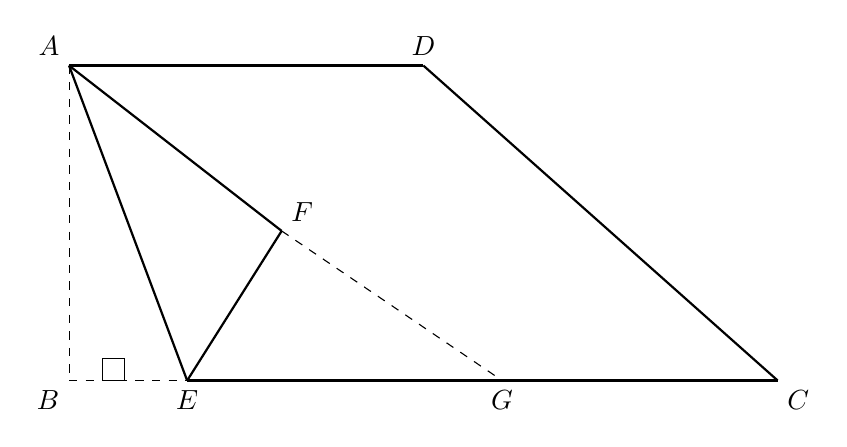
\begin{tikzpicture}
\coordinate (A) at (0,4);
\coordinate (B) at (0,0);
\coordinate (E) at (1.5,0);
\coordinate (F) at (2.7,1.9);
\coordinate (G) at (5.5,0);
\coordinate (C) at (9,0);
\coordinate (D) at (4.5,4);

\draw[dashed] (A) -- (B);
\draw[dashed] (B) -- (E);
\draw[dashed] (F) -- (G);
\draw[thick] (A) -- (D);
\draw[thick] (D) -- (C);
\draw[thick] (C) -- (E);
\draw[thick] (A) -- (F);
\draw[thick] (F) -- (E);
\draw[thick] (E) -- (A);

\draw ($(B)!0.28!(E)$) rectangle ++(0.28,0.28);

\node[above left] at (A) {$A$};
\node[below left] at (B) {$B$};
\node[below] at (E) {$E$};
\node[above right] at (F) {$F$};
\node[below] at (G) {$G$};
\node[below right] at (C) {$C$};
\node[above] at (D) {$D$};
\end{tikzpicture}
\end{document}
